% Options for packages loaded elsewhere
\PassOptionsToPackage{unicode}{hyperref}
\PassOptionsToPackage{hyphens}{url}
\PassOptionsToPackage{dvipsnames,svgnames*,x11names*,table}{xcolor}
%
\documentclass[
  13pt,
  %% For koma-script
  fontsize=13pt,
  russian,
  a4paper,
,captions=tableheading
]{scrreprt}
\usepackage{amsmath,amssymb}
\usepackage{lmodern}
\usepackage{setspace}
\usepackage{ifxetex,ifluatex}
\ifnum 0\ifxetex 1\fi\ifluatex 1\fi=0 % if pdftex
  \usepackage[T1]{fontenc}
  \usepackage[utf8]{inputenc}
  \usepackage{textcomp} % provide euro and other symbols
\else % if luatex or xetex
  \usepackage{unicode-math}
  \defaultfontfeatures{Scale=MatchLowercase}
  \defaultfontfeatures[\rmfamily]{Ligatures=TeX,Scale=1}
  \setmainfont[Ligatures=TeX]{PT Serif}
  \setsansfont[Ligatures=TeX,Scale=MatchLowercase]{PT Sans}
  \setmonofont[Scale=MatchLowercase,Contextuals=Alternate,Scale=0.8]{JuliaMono-Medium}
\fi
% koma-script tuning
\KOMAoptions{twoside=false}
\KOMAoptions{headings=standardclasses}
\KOMAoptions{headings=small}
\KOMAoptions{chapterprefix=false}
\renewcommand*{\chapterheadstartvskip}{}
% \renewcommand*{\chapterheadendvskip}{\vspace*{2\baselineskip}}
% \renewcommand{\chapterheadstartvskip}{\vspace*{10\baselineskip}}%
\RedeclareSectionCommand[beforeskip=0pt]{chapter}
% \RedeclareSectionCommand[%
% runin=false,
% afterindent=false,
% beforeskip=0pt,
% afterskip=0pt,
% afterskip=2\baselineskip,
% innerskip=0pt,
% ]{chapter}
% \RedeclareSectionCommand[%
% % runin=false,
% afterindent=false,
% beforeskip=\baselineskip,
% afterskip=.5\baselineskip]{section}
% \RedeclareSectionCommand[%
% % runin=false,
% afterindent=false,
% beforeskip=.75\baselineskip,
% afterskip=.5\baselineskip]{subsection}
% \RedeclareSectionCommand[%
% % runin=false,
% afterindent=false,
% beforeskip=.5\baselineskip,
% afterskip=.25\baselineskip]{subsubsection}
% \RedeclareSectionCommand[%
% runin=true,
% % afterindent=false,
% beforeskip=.5\baselineskip,
% afterskip=1em]{paragraph}
% \RedeclareSectionCommand[%
% runin=true,
% % afterindent=false,
% beforeskip=.5\baselineskip,
% afterskip=1em]{subparagraph}
% \setcaptionalignment[figure]{C}
% \setcaptionalignment[table]{R}
% \renewcommand*{\figureformat}{\figurename~\thefigure\autodot}
% \renewcommand*{\tableformat}{\tablename~\thetable\autodot}
\usepackage{enumitem}
\setlist{nosep}
\renewcommand{\labelitemi}{\bfseries\textemdash}                                                                                                                                                                                               
\renewcommand{\labelitemii}{\bfseries\textemdash}                                                                                                                                                                                              
\renewcommand{\labelitemiii}{\bfseries\textemdash}                                                                                                                                                                                             
\renewcommand{\labelitemiv}{\bfseries\textemdash}
%%
% Use upquote if available, for straight quotes in verbatim environments
\IfFileExists{upquote.sty}{\usepackage{upquote}}{}
\IfFileExists{microtype.sty}{% use microtype if available
  \usepackage[]{microtype}
  \UseMicrotypeSet[protrusion]{basicmath} % disable protrusion for tt fonts
}{}
\usepackage{indentfirst}
\usepackage{xcolor}
\definecolor{default-linkcolor}{HTML}{A50000}
\definecolor{default-filecolor}{HTML}{A50000}
\definecolor{default-citecolor}{HTML}{4077C0}
\definecolor{default-urlcolor}{HTML}{4077C0}
\IfFileExists{xurl.sty}{\usepackage{xurl}}{} % add URL line breaks if available
\IfFileExists{bookmark.sty}{\usepackage{bookmark}}{\usepackage{hyperref}}
\hypersetup{
  pdftitle={Имитационное моделирование сети передачи данных в Mininet},
  pdfauthor={С. М. Наливайко},
  pdflang={ru-RU},
  hidelinks,
  breaklinks=true,
  pdfcreator={LaTeX via pandoc with the Eisvogel template}}
\urlstyle{same} % disable monospaced font for URLs
\usepackage[left=30mm,right=15mm,top=20mm,bottom=20mm,nohead,includefoot=true]{geometry}

% % \AfterCalculatingTypearea{
%   \newgeometry{%
%   left=30mm,
%   right=15mm,
%   top=20mm,
%   bottom=20mm,
%   % bindingoffset=10mm,
%   % includefoot,
%   % foot=\baselineskip,
%   % showframe
% }
% % }
% % \recalctypearea


% add backlinks to footnote references, cf. https://tex.stackexchange.com/questions/302266/make-footnote-clickable-both-ways
\usepackage{footnotebackref}
\usepackage{graphicx}
\makeatletter
\def\maxwidth{\ifdim\Gin@nat@width>\linewidth\linewidth\else\Gin@nat@width\fi}
\def\maxheight{\ifdim\Gin@nat@height>\textheight\textheight\else\Gin@nat@height\fi}
\makeatother
% Scale images if necessary, so that they will not overflow the page
% margins by default, and it is still possible to overwrite the defaults
% using explicit options in \includegraphics[width, height, ...]{}
\setkeys{Gin}{width=\maxwidth,height=\maxheight,keepaspectratio}
% Set default figure placement to htbp
\makeatletter
\def\fps@figure{htbp}
\makeatother
\setlength{\emergencystretch}{3em} % prevent overfull lines
\providecommand{\tightlist}{%
  \setlength{\itemsep}{0pt}\setlength{\parskip}{0pt}}
\setcounter{secnumdepth}{5}

% Make use of float-package and set default placement for figures to H.
% The option H means 'PUT IT HERE' (as  opposed to the standard h option which means 'You may put it here if you like').
\usepackage{float}
\floatplacement{figure}{H}

\linepenalty=10
\interlinepenalty=0
\hyphenpenalty=50
\exhyphenpenalty=50
\binoppenalty=700
\relpenalty=500
\clubpenalty=150
\widowpenalty=150
\displaywidowpenalty=50
\brokenpenalty=100
\predisplaypenalty=10000
\postdisplaypenalty=0
\floatingpenalty = 20000
\flushbottom
\usepackage{float}
\floatplacement{figure}{!h}
\usepackage{menukeys}
\usepackage{minted}
\usepackage{amsmath}
\usepackage{mathtools}
\usepackage{physics}
\setminted{breaklines}
\graphicspath{{/}{image/}}
\makeatletter
\let\listoflistings\@undefined
\makeatother
\makeatletter
\@ifpackageloaded{subfig}{}{\usepackage{subfig}}
\@ifpackageloaded{caption}{}{\usepackage{caption}}
\captionsetup[subfloat]{margin=0.5em}
\AtBeginDocument{%
\renewcommand*\figurename{Figure}
\renewcommand*\tablename{Table}
}
\AtBeginDocument{%
\renewcommand*\listfigurename{List of Figures}
\renewcommand*\listtablename{List of Tables}
}
\newcounter{pandoccrossref@subfigures@footnote@counter}
\newenvironment{pandoccrossrefsubfigures}{%
\setcounter{pandoccrossref@subfigures@footnote@counter}{0}
\begin{figure}\centering%
\gdef\global@pandoccrossref@subfigures@footnotes{}%
\DeclareRobustCommand{\footnote}[1]{\footnotemark%
\stepcounter{pandoccrossref@subfigures@footnote@counter}%
\ifx\global@pandoccrossref@subfigures@footnotes\empty%
\gdef\global@pandoccrossref@subfigures@footnotes{{##1}}%
\else%
\g@addto@macro\global@pandoccrossref@subfigures@footnotes{, {##1}}%
\fi}}%
{\end{figure}%
\addtocounter{footnote}{-\value{pandoccrossref@subfigures@footnote@counter}}
\@for\f:=\global@pandoccrossref@subfigures@footnotes\do{\stepcounter{footnote}\footnotetext{\f}}%
\gdef\global@pandoccrossref@subfigures@footnotes{}}
\@ifpackageloaded{float}{}{\usepackage{float}}
\floatstyle{ruled}
\@ifundefined{c@chapter}{\newfloat{codelisting}{h}{lop}}{\newfloat{codelisting}{h}{lop}[chapter]}
\floatname{codelisting}{Listing}
\newcommand*\listoflistings{\listof{codelisting}{List of Listings}}
\makeatother
\iftutex
      % Load polyglossia as late as possible: uses bidi with RTL langages (e.g. Hebrew, Arabic)
  \usepackage{polyglossia}
  \setmainlanguage[spelling=modern,babelshorthands=true]{russian}
  \setotherlanguage[]{english}
\else
  \usepackage[main=russian]{babel}
% get rid of language-specific shorthands (see #6817):
\let\LanguageShortHands\languageshorthands
\def\languageshorthands#1{}
\fi
\ifluatex
  \usepackage{selnolig}  % disable illegal ligatures
\fi
\usepackage[style=gost-numeric,parentracker=true,backend=biber,hyperref=auto,language=auto,autolang=other*,citestyle=gost-numeric]{biblatex}
\addbibresource{bib/cite.bib}

\title{Имитационное моделирование сети передачи данных в Mininet}
\author{С. М. Наливайко}
\date{}



%%
%% added
%%

%
% language specification
%
% If no language is specified, use English as the default main document language.
%



%
% for the background color of the title page
%

%
% break urls
%
\PassOptionsToPackage{hyphens}{url}

%
% When using babel or polyglossia with biblatex, loading csquotes is recommended
% to ensure that quoted texts are typeset according to the rules of your main language.
%
\usepackage{csquotes}

%
% captions
%
% \definecolor{caption-color}{HTML}{777777}
% \usepackage[font={stretch=1.2}, textfont={color=caption-color}, position=top, skip=4mm, labelfont=bf, singlelinecheck=false, labelsep=space, justification=raggedright]{caption}
\usepackage[font={stretch=1.2}, position=top, skip=4mm, labelfont=bf,
singlelinecheck=false, labelsep=space,
justification=raggedright]{caption}
\captionsetup{font={small}}
\captionsetup{textfont={bf},labelfont={bf}}
% \DeclareCaptionFormat{tableRight}{\hfill#1\newline#2#3\par}
\DeclareCaptionFormat{gost1.5}{\hfill#1\newline#2#3\par}
\captionsetup[figure]{labelsep=space,position=bottom,justification=centering}
% \captionsetup[table]{format=tableRight,labelsep=none,position=top}
\captionsetup[table]{format=gost1.5,labelsep=none,position=top,justification=centering}
% \setcapindent{0em}

%
% blockquote
%
\definecolor{blockquote-border}{RGB}{221,221,221}
\definecolor{blockquote-text}{RGB}{119,119,119}
\usepackage{mdframed}
\newmdenv[rightline=false,bottomline=false,topline=false,linewidth=3pt,linecolor=blockquote-border,skipabove=\parskip]{customblockquote}
\renewenvironment{quote}{\begin{customblockquote}\list{}{\rightmargin=0em\leftmargin=0em}%
\item\relax\color{blockquote-text}\ignorespaces}{\unskip\unskip\endlist\end{customblockquote}}

%
% Source Sans Pro as the de­fault font fam­ily
% Source Code Pro for monospace text
%
% 'default' option sets the default
% font family to Source Sans Pro, not \sfdefault.
%
\ifnum 0\ifxetex 1\fi\ifluatex 1\fi=0 % if pdftex
    \usepackage[default]{sourcesanspro}
  \usepackage{sourcecodepro}
  \else % if not pdftex
    \fi

%
% heading color
%
\definecolor{heading-color}{RGB}{40,40,40}
\addtokomafont{section}{\color{heading-color}}
% When using the classes report, scrreprt, book,
% scrbook or memoir, uncomment the following line.
\addtokomafont{chapter}{\color{heading-color}}

%
% variables for title, author and date
%
\usepackage{titling}
\title{Имитационное моделирование сети передачи данных в Mininet}
\author{С. М. Наливайко}
\date{}

%
% tables
%

%
% remove paragraph indention
%
% \setlength{\parindent}{0pt}
% \setlength{\parskip}{6pt plus 2pt minus 1pt}
% \setlength{\emergencystretch}{3em}  % prevent overfull lines

%
%
% Listings
%
%


%
% header and footer
%

%%
%% end added
%%

\begin{document}

%%
%% begin titlepage
%%

\begin{titlepage}
  \newgeometry{top=2cm, right=1.5cm, bottom=2cm, left=3cm}

  % % \AtBeginDocument{%
  % \makeatletter
  % \@ifpackageloaded{polyglossia}{%
  %   \addto\captionsrussian@modern{%
  %     \def\PHDauthorDescr{Выполнил студент}
  %     \def\PHDstudygroupDescr{Группа}
  %     % \def\PHDstudygroupDescr{Студент группы}
  %     \def\PHDcountryDescr{Страна}
  %     % \def\PHDchiefDescr{Научный руководитель}
  %     \def\PHDchiefDescr{Руководитель выпускной квалификационной работы}
  %     \def\PHDyearShort{г.}
  %     \def\PHDapprove{«Допустить к защите»}
  %     \def\PHDstudentdegreeDescr{Квалификация (степень)}
  %     \def\PHDstudentidDescr{Студенческий билет №}
  %     \def\PHDdegreeDescr{Квалификация (степень):}
  %     \def\PHDfieldDescr{Направление}
  %   }
  % }{%
  %   \def\PHDauthorDescr{{\CYRV}{\cyrery}{\cyrp}{\cyro}{\cyrl}{\cyrn}{\cyri}{\cyrl} {\cyrs}{\cyrt}{\cyru}{\cyrd}{\cyre}{\cyrn}{\cyrt}}
  %   \def\PHDstudygroupDescr{\cyr\CYRG\cyrr\cyru\cyrp\cyrp\cyra{}}
  %   % \def\PHDstudygroupDescr{{\CYRS}{\cyrt}{\cyru}{\cyrd}{\cyre}{\cyrn}{\cyrt} {\cyrg}{\cyrr}{\cyru}{\cyrp}{\cyrp}{\cyrery}}
  %   \def\PHDcountryDescr{\cyr\CYRS\cyrt\cyrr\cyra\cyrn\cyra{}}
  %   % \def\PHDchiefDescr{\cyr\CYRN\cyra\cyru\cyrch\cyrn\cyrery\cyrishrt{}
  %   % \cyr\cyrr\cyru\cyrk\cyro\cyrv\cyro\cyrd\cyri\cyrt\cyre\cyrl\cyrsftsn{}}
  %   \def\PHDchiefDescr{{\CYRR}{\cyru}{\cyrk}{\cyro}{\cyrv}{\cyro}{\cyrd}{\cyri}{\cyrt}{\cyre}{\cyrl}{\cyrsftsn}
  %     {\cyrv}{\cyrery}{\cyrp}{\cyru}{\cyrs}{\cyrk}{\cyrn}{\cyro}{\cyrishrt}
  %     {\cyrk}{\cyrv}{\cyra}{\cyrl}{\cyri}{\cyrf}{\cyri}{\cyrk}{\cyra}{\cyrc}{\cyri}{\cyro}{\cyrn}{\cyrn}{\cyro}{\cyrishrt} {\cyrr}{\cyra}{\cyrb}{\cyro}{\cyrt}{\cyrery}}
  %   \def\PHDyearShort{\cyrg.}
  %   \def\PHDapprove{<<{\CYRD}{\cyro}{\cyrp}{\cyru}{\cyrs}{\cyrt}{\cyri}{\cyrt}{\cyrsftsn} {\cyrk} {\cyrz}{\cyra}{\cyrshch}{\cyri}{\cyrt}{\cyre}>>}
  %   \def\PHDstudentdegreeDescr{{\CYRK}{\cyrv}{\cyra}{\cyrl}{\cyri}{\cyrf}{\cyri}{\cyrk}{\cyra}{\cyrc}{\cyri}{\cyrya}
  %     ({\cyrs}{\cyrt}{\cyre}{\cyrp}{\cyre}{\cyrn}{\cyrsftsn})}
  %   \def\PHDstudentidDescr{{\CYRS}{\cyrt}{\cyru}{\cyrd}{\cyre}{\cyrn}{\cyrch}{\cyre}{\cyrs}{\cyrk}{\cyri}{\cyrishrt}
  %     {\cyrb}{\cyri}{\cyrl}{\cyre}{\cyrt} \No{}}
  %   \def\PHDdegreeDescr{{\CYRK}{\cyrv}{\cyra}{\cyrl}{\cyri}{\cyrf}{\cyri}{\cyrk}{\cyra}{\cyrc}{\cyri}{\cyrya}
  %     ({\cyrs}{\cyrt}{\cyre}{\cyrp}{\cyre}{\cyrn}{\cyrsftsn}):}
  %   \def\PHDfieldDescr{{\CYRN}{\cyra}{\cyrp}{\cyrr}{\cyra}{\cyrv}{\cyrl}{\cyre}{\cyrn}{\cyri}{\cyre}}
  % }
  % \makeatother
  % % }

  \providecommand{\approvedStamp}{%
    \begin{flushright}
      \begin{minipage}[t]{0.4\linewidth}
        \begin{flushright}
          \MakeUppercase{Утверждаю}
        \end{flushright}
        \smallskip
        \begin{flushright}
          {Заведующий кафедрой прикладной информатики и теории
вероятностей} \\
          {д.т.н., профессор} \\
          \hrulefill{}
          {К. Е. Самуйлов} \\
          \smallskip
          <<\underline{\ \ \ \ \ \ }>>
          \hrulefill{}
          20\underline{\ \ \ \ }~г.
        \end{flushright}
      \end{minipage}
    \end{flushright}
  }
  
  \providecommand{\authorTable}{%
    % Автор
    \noindent
    \hfill
    \begin{minipage}[t]{0.5\linewidth}
      % Группа
            Выполнил \par
      \medskip
      {Студент группы}
      {НФИбд-01-18} \par
      \medskip
            % Студбилет
            % Автор
            \hrulefill{}
      С. М. Наливайко\par
      <<\underline{\ \ \ \ \ \ }>>
      \hrulefill{}
      20\underline{\ \ \ \ }~г.
      \par
            \bigskip
      \bigskip
      %% Научный руководитель
            Руководитель \par
      \medskip
      {доцент кафедры прикладной информатики и теории вероятностей} \par
      {к.ф.-м.н., доцент} \par
      \hrulefill{}
      {А. В. Королькова}
          \end{minipage}
  }

  \thispagestyle{empty}
  \setcounter{page}{1}
  \null\vfil
  \begin{center}
    % {\small \bfseries \MakeUppercase{\PHDministry} \par}
    % \smallskip
        {% \bfseries
      \MakeUppercase{Российский университет дружбы народов} \par}
    \smallskip
        % \hrule
    % \smallskip
    %% факультет
        {% \bfseries
      {Факультет физико-математических и естественных наук} \par}
        %% Кафедра
        {% \bfseries
      {Кафедра прикладной информатики и теории вероятностей} \par}
      \end{center}

  \bigskip
  \bigskip

  %% Approved stamp
  \approvedStamp

  \bigskip
  \bigskip

  \begin{center}
  
        \MakeUppercase{Курсовая работа} \par
    \smallskip
            на тему \par
    \smallskip
            <<Имитационное моделирование сети передачи данных в
Mininet>>\par
    \smallskip
        % По дисциплине (для реферата)
        \medskip%
    по дисциплине
    <<Компьютерный практикум по математическому моделированию>>
    \bigskip
      \end{center}

  \vspace{\fill}
  
  \bigskip%
  \authorTable


  \begin{center}
    \vspace*{\fill}
    % \bfseries
    % Город
    {Москва}
    {2021}
  \end{center}
  
\end{titlepage}
\restoregeometry

%%
%% end titlepage
%%



\renewcommand*\contentsname{Содержание}
{
\setcounter{tocdepth}{2}
\tableofcontents
}
\listoffigures
\setstretch{1.5}
\hypertarget{ux441ux43fux438ux441ux43eux43a-ux438ux441ux43fux43eux43bux44cux437ux443ux435ux43cux44bux445-ux441ux43eux43aux440ux430ux449ux435ux43dux438ux439}{%
\chapter*{Список используемых
сокращений}\label{ux441ux43fux438ux441ux43eux43a-ux438ux441ux43fux43eux43bux44cux437ux443ux435ux43cux44bux445-ux441ux43eux43aux440ux430ux449ux435ux43dux438ux439}}
\addcontentsline{toc}{chapter}{Список используемых сокращений}

\hypertarget{ux440ux443ux441ux441ux43aux43eux44fux437ux44bux447ux43dux44bux435-ux441ux43eux43aux440ux430ux449ux435ux43dux438ux44f}{%
\section*{Русскоязычные
сокращения}\label{ux440ux443ux441ux441ux43aux43eux44fux437ux44bux447ux43dux44bux435-ux441ux43eux43aux440ux430ux449ux435ux43dux438ux44f}}
\addcontentsline{toc}{section}{Русскоязычные сокращения}

ОС --- Операционная система

\hypertarget{ux430ux43dux433ux43bux43eux44fux437ux44bux447ux43dux44bux435-ux441ux43eux43aux440ux430ux449ux435ux43dux438ux44f}{%
\section*{Англоязычные
сокращения}\label{ux430ux43dux433ux43bux43eux44fux437ux44bux447ux43dux44bux435-ux441ux43eux43aux440ux430ux449ux435ux43dux438ux44f}}
\addcontentsline{toc}{section}{Англоязычные сокращения}

AMD --- Advanced Micro Devices

CBQ --- Class Based Queueing

CLI --- Сommand-Line Interface

HTB --- Hierarchy Token Bucket

IP --- Internet Protocol

JSON --- JavaScript Object Notation

PID --- Process Identity Document

QoS --- Quality of Service

RED --- Random Early Detection

RTT --- Round-Trip Time

SCTP --- Stream Control Transmission Protocol

SFQ --- Stochastic Fairness Queueing

SSD --- Solid-State Drive

TBF --- Token Bucket Filter

TCP --- Transmission Control Protocol

UDP --- User Datagram Protocol

\hypertarget{ux432ux432ux435ux434ux435ux43dux438ux435}{%
\chapter*{Введение}\label{ux432ux432ux435ux434ux435ux43dux438ux435}}
\addcontentsline{toc}{chapter}{Введение}

\(\quad\)Актуальной темы обусловлена потребностью организаций в
грамотном проектировании и развертывании локальной сети предприятия.
Создание сети не может обходится без предварительного анализа и
прототипирования. Для данных задач могут использоваться современные
программы, которые позволяют создавать и испытывать сети без реальных
сетевых компонентов. Такое решение дешево в построении, а сбор данных
сетевых характеристик заметно ускоряется и упрощается.

Целью работы является изучение возможностей измерения сетевых
характеристик передачи данных без использования реальных сетевых
компонентов и варьирование сетевых протоколов для достижения наилучшей
производительности детерминированной сети.

Основные задачи моей работы:

\begin{enumerate}
\def\labelenumi{\arabic{enumi}.}
\tightlist
\item
  Построить имитационную модель простой сети передачи данных в Mininet
  \autocite{mininet}.
\item
  Измерить и визуализировать характеристики моделируемой сети передачи
  данных для качественной оценки производительности сети.
\item
  Оценить влияние различных комбинаций протоколов на общую
  производительность моделируемой сети при заданных сетевых
  характеристиках.
\end{enumerate}

Методами исследования предметной области являются наблюдение, сравнение
и измерение. Каждый из этих методов полезен на практике при построении
сетей.

Курсовая работа состоит из введения, трех разделов, посвященных
построению виртуальной сети, ее конфигурации и измерению сетевых
характеристик передачи данных, заключения и списка используемой
литературы.

Во введении кратко дается представление исследуемой области.

В первом разделе рассказывается о виртуальной среде Mininet, в которой
будет проводится исследование. Далее будет дан способ установки Mininet
на свою рабочую станцию и будет осуществлен первый запуск виртуальной
сети.

Во втором разделе дается представление о генерации трафика и его
передачи между хостами с помощью утилиты iPerf3 \autocite{iperf}. Будут
рассмотрены параметры запуска данной утилиты и способы визуализации
сетевых характеристик передачи данных, полученных данной утилитой.

В третьем разделе рассматривается утилита iproute2 \autocite{iproute},
которая помогает настраивать интерфейсы сетевых элементов. Далее
рассматриваются виды дисциплин очередей, настройка дисциплин очередей на
сетевых интерфейсах и получение статистических данных дисциплины с
помощью iproute2.

В заключении подведены основные выводы проделанной работы.

\hypertarget{ux43fux43eux441ux442ux440ux43eux435ux43dux438ux435-ux432ux438ux440ux442ux443ux430ux43bux44cux43dux43eux439-ux441ux435ux442ux438-ux441-ux43fux43eux43cux43eux449ux44cux44e-mininet}{%
\chapter{Построение виртуальной сети с помощью
Mininet}\label{ux43fux43eux441ux442ux440ux43eux435ux43dux438ux435-ux432ux438ux440ux442ux443ux430ux43bux44cux43dux43eux439-ux441ux435ux442ux438-ux441-ux43fux43eux43cux43eux449ux44cux44e-mininet}}

\hypertarget{ux43eux431ux449ux438ux435-ux441ux432ux435ux434ux435ux43dux438ux44f}{%
\section{Общие
сведения}\label{ux43eux431ux449ux438ux435-ux441ux432ux435ux434ux435ux43dux438ux44f}}

\(\quad\)Mininet \autocite{mininet} --- это виртуальная среда, которая
позволяет разрабатывать и тестировать сетевые инструменты и протоколы. В
сетях Mininet работают реальные сетевые приложения Unix/Linux, а также
реальное ядро Linux и сетевой стек. С помощью одной команды Mininet
может создать виртуальную сеть на любом типе машины, будь то виртуальная
машина, размещенная в облаке или же собственный персональный компьютер.
Это дает значительные плюсы при тестировании работоспособности
протоколов или сетевых программ:

\begin{itemize}
\tightlist
\item
  позволяет быстро создавать прототипы программно-определяемых сетей;
\item
  тестирование не требует экспериментов в реальной сетевой среде,
  вследствие чего разработка ведется быстрее;
\item
  тестирование в сложных сетевых топологиях обходится без необходимости
  покупать дорогое оборудование;
\item
  виртуальный эксперимент приближен к реальному, так как Mininet
  запускает код на реальном ядре Linux;
\item
  позволяет работать нескольким разработчикам в одной топологией
  независимо.
\end{itemize}

Машины (хосты) в сети создаются по образу машины, которая запускает
Mininet, со всеми вытекающими обстоятельствами. Например, если
количество памяти, допустимое для буфера передачи сокета TCP, на рабочей
машине равно, например, значению 4096MB, то и на виртуальной машине это
значение будет таким же. Изменение конфигурации на машине в виртуальной
сети не вносит изменений в конфигурацию рабочей машины.

\hypertarget{ux443ux441ux442ux430ux43dux43eux432ux43aux430-mininet}{%
\section{Установка
Mininet}\label{ux443ux441ux442ux430ux43dux43eux432ux43aux430-mininet}}

\hypertarget{ux443ux43aux430ux437ux430ux43dux438ux44f-ux43a-ux443ux441ux442ux430ux43dux43eux432ux43aux435}{%
\subsection{Указания к
установке}\label{ux443ux43aux430ux437ux430ux43dux438ux44f-ux43a-ux443ux441ux442ux430ux43dux43eux432ux43aux435}}

Описание выполнения установки приведено для техники со следующими
характеристиками:

\begin{itemize}
\tightlist
\item
  ОС ubuntu-20.04.3
\item
  AMD Ryzen 7 3700X 3600 MHz, 4Гб оперативной памяти, 20Гб свободно на
  SSD.
\end{itemize}

\hypertarget{ux43fux440ux43eux446ux435ux441ux441-ux443ux441ux442ux430ux43dux43eux432ux43aux438}{%
\subsection{Процесс
установки}\label{ux43fux440ux43eux446ux435ux441ux441-ux443ux441ux442ux430ux43dux43eux432ux43aux438}}

\begin{enumerate}
\def\labelenumi{\arabic{enumi}.}
\item
  Перейдем на сайт mininet.org.
\item
  Перейдем в раздел Download и выберем режим установки mininet. Mininet
  дает нам 3 опции по установке: установка образа посредством github,
  установка из исходного кода на персональный компьютер или установка
  пакетом для Ubuntu посредством apt. Мы выбрали второй вариант
  установки.
\item
  Установим исходный код программы mininet и перейдем в установленную
  директорию при помощи команды
\end{enumerate}

\begin{minted}[breaklines]{bash}
git clone git://github.com/mininet/mininet && cd mininet
\end{minted}

\begin{enumerate}
\def\labelenumi{\arabic{enumi}.}
\setcounter{enumi}{3}
\tightlist
\item
  Произведем установку программы mininet при помощи команды
\end{enumerate}

\begin{minted}[breaklines]{bash}
./util/install.sh -a
\end{minted}

Опция -a в команде означает, что мы хотим установить программу полностью
со всеми зависимостями (например POX, Open vSwitch, OpenFlow).

После установки в директории /usr/local/lib/pythonV/dist-packages
появится каталог mininet.

\begin{enumerate}
\def\labelenumi{\arabic{enumi}.}
\setcounter{enumi}{4}
\tightlist
\item
  Если в ходе установки не возникло ошибок, то можно запустить Mininet и
  проверить работоспособность при помощи команды
  \mintinline{bash}{sudo mn}.
\end{enumerate}

Вывод команды приведен на рис. \ref{fig:0001}. Mininet требует права
суперпользователя для запуска.

\begin{figure}
\hypertarget{fig:0001}{%
\centering
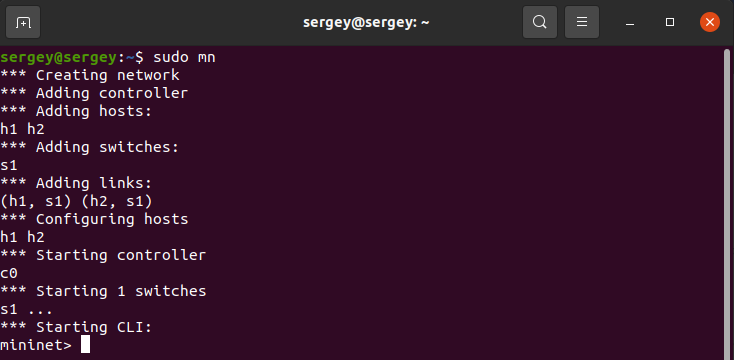
\includegraphics[width=0.7\textwidth,height=\textheight]{mininet_1.5.png}
\caption{Запуск Mininet}\label{fig:0001}
}
\end{figure}

\begin{enumerate}
\def\labelenumi{\arabic{enumi}.}
\setcounter{enumi}{5}
\tightlist
\item
  Удалим исходный код программы командой
  \mintinline{bash}{rm -rf mininet}.
\end{enumerate}

\hypertarget{ux440ux430ux431ux43eux442ux430-ux441-ux43fux440ux43eux433ux440ux430ux43cux43cux43eux439-mininet}{%
\section{Работа с программой
Mininet}\label{ux440ux430ux431ux43eux442ux430-ux441-ux43fux440ux43eux433ux440ux430ux43cux43cux43eux439-mininet}}

\(\quad\)После запуска Mininet посредством команды
\mintinline{bash}{sudo mn} у нас создастся простая сеть с хостами h1 и
h2 и коммутатором s1, который соединяет хосты между собой. Также хостам
были присвоены ip-адреса (10.0.0.1 для h1 и 10.0.0.2 для h2). Мы можем
проверить достижимость сетевых компонентов с помощью команды
\mintinline{bash}{h1 ping h2} посредством CLI или же запустить терминал
для хоста, например, h1 и выполнять всю работу из терминала, как на
реальном устройстве. Запуск терминала осуществляется командой
\mintinline{bash}{xterm h1} из CLI.

Проверим достижимость h2 для h1 из терминала можно с помощью команды
\mintinline{bash}{ping} (рис. \ref{fig:0002}).

\begin{figure}
\hypertarget{fig:0002}{%
\centering
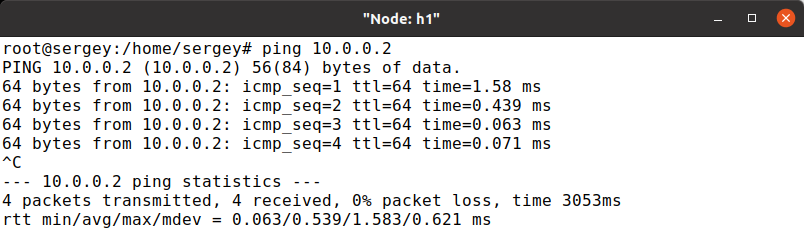
\includegraphics[width=0.7\textwidth,height=\textheight]{mininet_2.2.png}
\caption{Проверка достижимости h2 для h1}\label{fig:0002}
}
\end{figure}

Узнать список доступных команд Mininet можно в CLI с помощью команды
\mintinline{bash}{help}.

\hypertarget{miniedit}{%
\section{MiniEdit}\label{miniedit}}

\(\quad\)Mininet предоставляет графический интерфейс управления
виртуальной сетью --- MiniEdit. MiniEdit --- программа, написанная на
языке программирования Python, которая является надстройкой над mn и
позволяет управлять сетью в удобном для пользователя виде. Данная
программа расположена в директории examples исходных файлов mininet. В
моем случае это директория
/usr/local/lib/python3.8/dist-packages/mininet/examples/miniedit.py.

Создадим простую топологию из двух хостов и коммутатора в MiniEdit.

\begin{enumerate}
\def\labelenumi{\arabic{enumi}.}
\tightlist
\item
  Запустим Miniedit:
\end{enumerate}

\begin{minted}[breaklines]{bash}
sudo python3 /usr/local/lib/python3.8/dist-packages/mininet/examples/miniedit.py
\end{minted}

\begin{enumerate}
\def\labelenumi{\arabic{enumi}.}
\setcounter{enumi}{1}
\item
  Создадим 2 хоста, выбрав иконку терминала и кликнув по рабочей области
  2 раза. Имена для хостов присваиваются автоматически.
\item
  Кликнув правой кнопкой мыши по хосту и выбрав раздел Properties,
  зададим в поле IP-адреса 10.0.0.1 и 10.0.0.2 соответственно (рис.
  \ref{fig:0003}).
\end{enumerate}

\begin{figure}
\hypertarget{fig:0003}{%
\centering
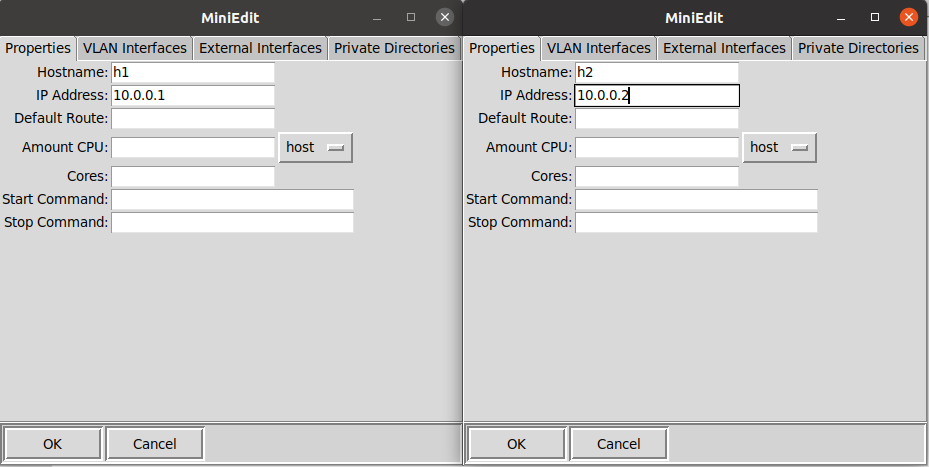
\includegraphics[width=0.7\textwidth,height=\textheight]{mininet_2.3.png}
\caption{Редактирование конфигурации хостов сети}\label{fig:0003}
}
\end{figure}

\begin{enumerate}
\def\labelenumi{\arabic{enumi}.}
\setcounter{enumi}{3}
\item
  Добавим в рабочую область коммутатор, выбрав элемент LegacySwitch.
\item
  Выберем элемент NetLink и соединим элементы сети (рис.
  \ref{fig:0004}).
\end{enumerate}

\begin{figure}
\hypertarget{fig:0004}{%
\centering
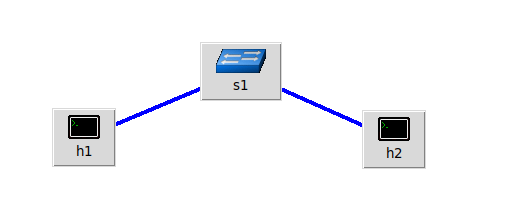
\includegraphics[width=0.7\textwidth,height=\textheight]{mininet_2.4.png}
\caption{Соединение элементов сети}\label{fig:0004}
}
\end{figure}

\begin{enumerate}
\def\labelenumi{\arabic{enumi}.}
\setcounter{enumi}{5}
\item
  Запустим сеть, нажав на кнопку Run.
\item
  Откроем терминал первого хоста, нажав правой кнопкой мыши по хосту и
  выбрав пункт Terminal. Отправим \mintinline{bash}{ping} второму хосту
  (рис. \ref{fig:0005}).
\end{enumerate}

\begin{figure}
\hypertarget{fig:0005}{%
\centering
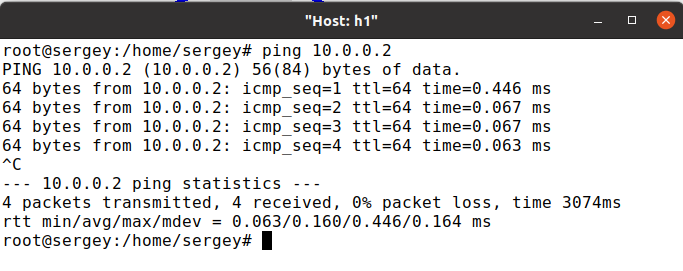
\includegraphics[width=0.7\textwidth,height=\textheight]{mininet_2.5.png}
\caption{Проверка достижимости h2 для h1}\label{fig:0005}
}
\end{figure}

\hypertarget{ux433ux435ux43dux435ux440ux430ux446ux438ux44f-ux438-ux438ux437ux43cux435ux440ux435ux43dux438ux435-ux441ux435ux442ux435ux432ux43eux433ux43e-ux442ux440ux430ux444ux438ux43aux430-ux441-ux43fux43eux43cux43eux449ux44cux44e-ux443ux442ux438ux43bux438ux442ux44b-iperf3}{%
\chapter{Генерация и измерение сетевого трафика с помощью утилиты
iPerf3}\label{ux433ux435ux43dux435ux440ux430ux446ux438ux44f-ux438-ux438ux437ux43cux435ux440ux435ux43dux438ux435-ux441ux435ux442ux435ux432ux43eux433ux43e-ux442ux440ux430ux444ux438ux43aux430-ux441-ux43fux43eux43cux43eux449ux44cux44e-ux443ux442ux438ux43bux438ux442ux44b-iperf3}}

\hypertarget{ux43eux431ux449ux438ux435-ux441ux432ux435ux434ux435ux43dux438ux44f}{%
\section{Общие
сведения}\label{ux43eux431ux449ux438ux435-ux441ux432ux435ux434ux435ux43dux438ux44f}}

\(\quad\)iPerf3 \autocite{iperf} --- кроссплатформенная консольная
клиент-серверная программа-генератор TCP, UDP и SCTP трафика для
тестирования пропускной способности сети. По умолчанию тест выполняется
в направлении от клиента к серверу. Для выполнения тестирования
программа должна быть запущена на двух устройствах (это могут быть как
компьютеры, так и смартфоны, планшеты). Одно из них будет выполнять роль
сервера, а другое роль клиента. Между ними и будет происходить передача
данных для измерения пропускной способности соединения.

\hypertarget{ux442ux435ux441ux442ux438ux440ux43eux432ux430ux43dux438ux435-ux43fux440ux43eux43fux443ux441ux43aux43dux43eux439-ux441ux43fux43eux441ux43eux431ux43dux43eux441ux442ux438-ux441-ux43fux43eux43cux43eux449ux44cux44e-iperf3}{%
\section{Тестирование пропускной способности с помощью
iPerf3}\label{ux442ux435ux441ux442ux438ux440ux43eux432ux430ux43dux438ux435-ux43fux440ux43eux43fux443ux441ux43aux43dux43eux439-ux441ux43fux43eux441ux43eux431ux43dux43eux441ux442ux438-ux441-ux43fux43eux43cux43eux449ux44cux44e-iperf3}}

\(\quad\)Для запуска сервера iPerf требуется выполнить следующую команду

\begin{minted}[breaklines]{bash}
iPerf3 -s [параметры]
\end{minted}

Список параметров для сервера:

\begin{itemize}
\tightlist
\item
  -D, --daemon (запуск сервера как процесс демон);
\item
  -I, --pidfile file (ведется запись в PID-файл);
\item
  -1, --one-off (после обслуживания 1 клиента работа сервера
  прекращается).
\end{itemize}

Для запуска iPerf-клиента требуется выполнить следующую команду:

\begin{minted}[breaklines]{bash}
iPerf3 -c server_ip [параметры]
\end{minted}

Список параметров для клиента:

\begin{itemize}
\tightlist
\item
  -u, --udp (используется);
\item
  -b, --bandwidth (указывает пропускную способность);
\item
  -t, --time (время передачи);
\item
  -n, --bytes (количество байтов для передачи);
\item
  -k, --blockcount (количество блоков данных для передачи);
\item
  -l, --len (размер буфера для передачи/приема);
\item
  -cport (указание порта передачи для клиента);
\item
  -P, --parallel (количество потоков передачи);
\item
  -R, --reverse (указание поменять сервер и клиент местами);
\item
  -w, --window (изменение размера окна TCP);
\item
  -M, --set-mss (изменение максимального размера сегмента);
\item
  -N, --no-delay (удалить задержку в TCP/SCTP);
\item
  -4, --version4 (использовать только ipv4);
\item
  -6, --version6 (использовать только ipv6);
\item
  -S, --tos N (установить тип услуги);
\item
  -Z, --zerocopy (использовать метод отправки данных с нулевой копией);
\item
  -O, --omit N (опустить первые n секунд передачи при статистике);
\item
  -T, --title str (префикс каждой выходной строки с этой строкой);
\item
  -get-server-output (получение результатов от сервера);
\item
  --udp-counters-64bit (использовать 64-битные счетчики в тестовых
  пакетах UDP).
\end{itemize}

Общие параметры для сервера и клиента:

\begin{itemize}
\tightlist
\item
  -p, --port (порт для прослушивания);
\item
  -f, --format (формат статистики: Мбит, Кбит \ldots);
\item
  -i, --interval (интервалы между замерами);
\item
  -F, --file name (xmit/recv файл);
\item
  -B, --bind (связать определенный интерфейс);
\item
  -V, --verbose (более детальная статистика);
\item
  -J, --json (вывод статистики в json- файл);
\item
  --logfile f (отправить данные в лог-файл);
\item
  -d, --debug (выдать отладочную информацию);
\item
  -v, --version (показать версию программы и выйти);
\item
  -h, --help (показать help-информацию и выйти).
\end{itemize}

Проведем тестирование сети в Mininet:

\begin{enumerate}
\def\labelenumi{\arabic{enumi}.}
\tightlist
\item
  Запустим MiniEdit, создадим два хоста (h1 и h2) и коммутатор (s1),
  соединим элементы сети, запустим сеть (рис. \ref{fig:0011}).
\end{enumerate}

\begin{figure}
\hypertarget{fig:0011}{%
\centering
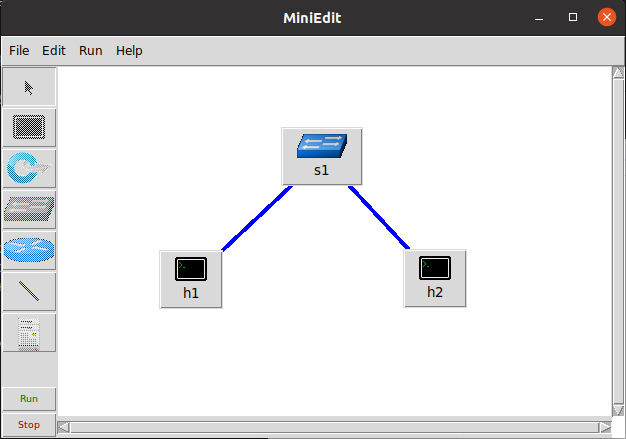
\includegraphics[width=0.7\textwidth,height=\textheight]{iperf_1.png}
\caption{Сеть с простой топологией в Mininet}\label{fig:0011}
}
\end{figure}

\begin{enumerate}
\def\labelenumi{\arabic{enumi}.}
\setcounter{enumi}{1}
\tightlist
\item
  Запустим iPerf-сервер на h2, введя в терминале этого устройства
  команду
\end{enumerate}

\begin{minted}[breaklines]{bash}
iper3 -s
\end{minted}

\begin{enumerate}
\def\labelenumi{\arabic{enumi}.}
\setcounter{enumi}{2}
\tightlist
\item
  Запустим iPerf-клиент на хосте h1 на 60 секунд, пропустив первые 10
  секунд для статистики (рис. \ref{fig:0012}):
\end{enumerate}

\begin{minted}[breaklines]{bash}
iPerf3 -c 10.0.0.2 -t 60 -O 10
\end{minted}

\begin{figure}
\hypertarget{fig:0012}{%
\centering
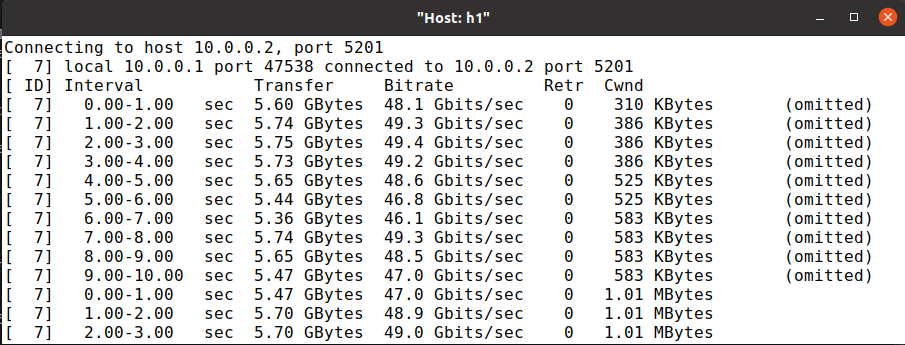
\includegraphics[width=0.7\textwidth,height=\textheight]{iperf_3.png}
\caption{Запуск iPerf-клиента}\label{fig:0012}
}
\end{figure}

\begin{enumerate}
\def\labelenumi{\arabic{enumi}.}
\setcounter{enumi}{3}
\tightlist
\item
  Просмотрим статистику, которую сгенерировал iPerf (рис.
  \ref{fig:0013}).
\end{enumerate}

\begin{figure}
\hypertarget{fig:0013}{%
\centering
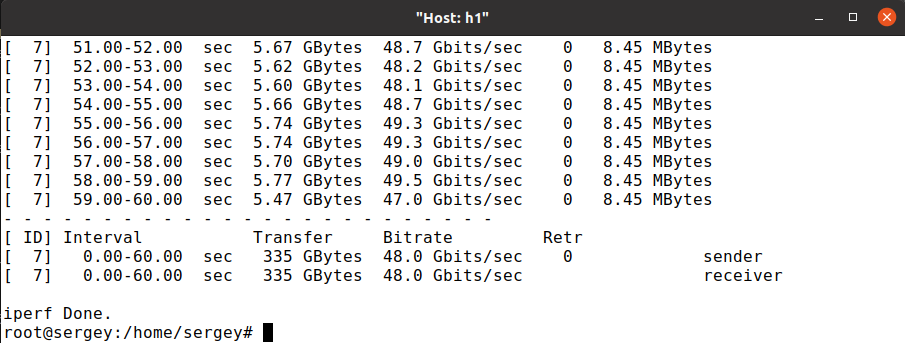
\includegraphics[width=0.7\textwidth,height=\textheight]{iperf_4.png}
\caption{Вывод статистики iPerf3}\label{fig:0013}
}
\end{figure}

\hypertarget{ux43fux43eux441ux442ux440ux43eux435ux43dux438ux435-ux433ux440ux430ux444ux438ux43aux43eux432-ux441ux435ux442ux435ux432ux44bux445-ux445ux430ux440ux430ux43aux442ux435ux440ux438ux441ux442ux438ux43a}{%
\section{Построение графиков сетевых
характеристик}\label{ux43fux43eux441ux442ux440ux43eux435ux43dux438ux435-ux433ux440ux430ux444ux438ux43aux43eux432-ux441ux435ux442ux435ux432ux44bux445-ux445ux430ux440ux430ux43aux442ux435ux440ux438ux441ux442ux438ux43a}}

\(\quad\)iPerf3 предоставляет нам обширные количество данных, которые
можно исследовать. Наиболее удобным представлением данных сетевых
характеристик является графическое представление.

Для того, чтобы построить графики воспользуемся самописным скриптом
plotter.py, который подробно рассмотрен в
\protect\hyperlink{appendix1}{Приложении А}. Данный скрипт обрабатывает
файл json, который мы получаем в iPerf3, и на основе него строит
графики.

Визуализируем данные сетевой статистики.

\begin{enumerate}
\def\labelenumi{\arabic{enumi}.}
\tightlist
\item
  Воспользуемся виртуальной сетью из прошлого раздела.
\item
  Запустим iPerf-сервер на хосте h2.
\item
  Запустим iPerf3-клиент на хосте h1 с параметром -J, который формирует
  json-файл со статистикой:
\end{enumerate}

\begin{minted}[breaklines]{bash}
iPerf3 -c 10.0.0.2 -t 60 -J > data.json
\end{minted}

\begin{enumerate}
\def\labelenumi{\arabic{enumi}.}
\setcounter{enumi}{3}
\tightlist
\item
  Дождемся окончания передачи данных и запустим скрипт из
  \protect\hyperlink{appendix1}{Приложения А}:
\end{enumerate}

\begin{minted}[breaklines]{bash}
./plotter.py -i data.json
\end{minted}

В результате выполнения скрипта создается директория monitoring, в
которой находятся все статистические данных iPerf.

\begin{enumerate}
\def\labelenumi{\arabic{enumi}.}
\setcounter{enumi}{4}
\tightlist
\item
  Рассмотрим полученные графики:
\end{enumerate}

На рис. \ref{fig:0014} приведен график, показывающий динамику объема
переданных данных за время моделирования.

\begin{figure}
\hypertarget{fig:0014}{%
\centering
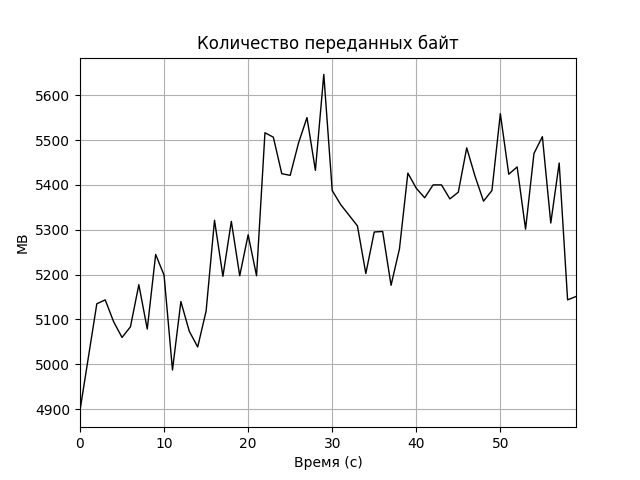
\includegraphics[width=0.7\textwidth,height=\textheight]{iperf_bytes.png}
\caption{График изменения количества переданных данных с течением
времени}\label{fig:0014}
}
\end{figure}

На рис. \ref{fig:0015} приведен график изменения значений окна
перегрузки протокола TCP Cubic (CWND).

\begin{figure}
\hypertarget{fig:0015}{%
\centering
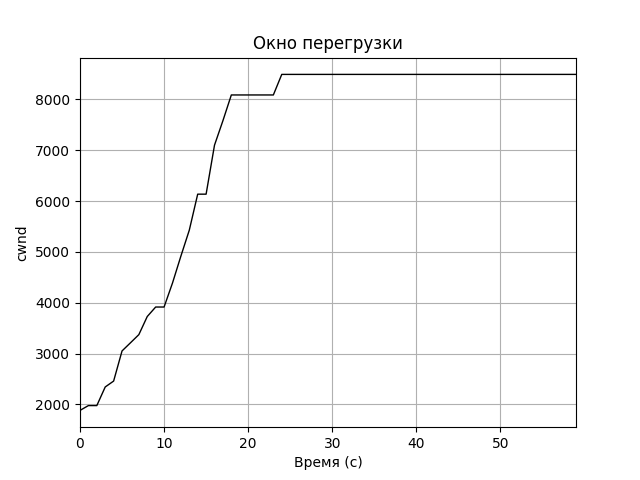
\includegraphics[width=0.7\textwidth,height=\textheight]{iperf_cwnd.png}
\caption{График изменения значения окна перегрузки с течением времени
при использовании алгоритма TCP Cubic}\label{fig:0015}
}
\end{figure}

Динамика значений RTT (измеряется в миллисекундах) демонстрируется на
рис \ref{fig:0017}.

\begin{figure}
\hypertarget{fig:0017}{%
\centering
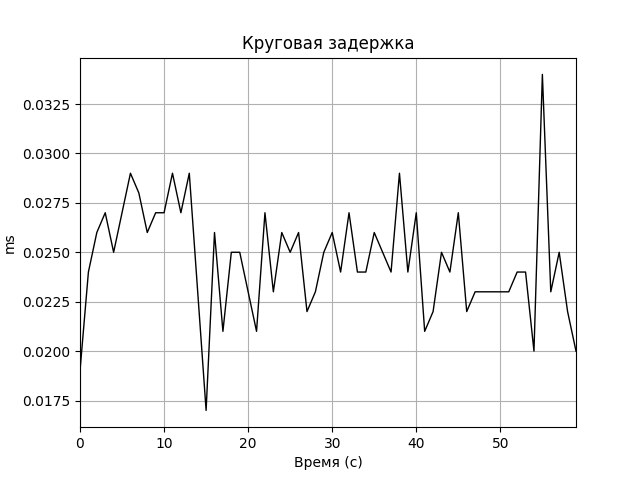
\includegraphics[width=0.7\textwidth,height=\textheight]{iperf_rtt.png}
\caption{График изменения значения RTT с течением
времени}\label{fig:0017}
}
\end{figure}

График отклонений значений RTT приведен на рис. \ref{fig:0018}.

\begin{figure}
\hypertarget{fig:0018}{%
\centering
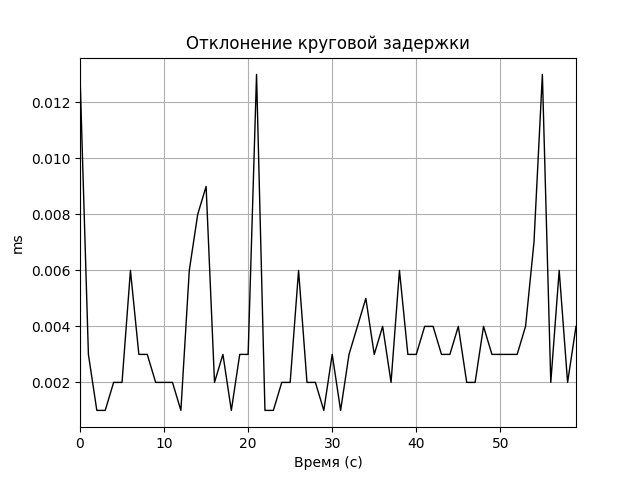
\includegraphics[width=0.7\textwidth,height=\textheight]{iperf_rttvar.png}
\caption{График изменения значения вариации RTT с течением
времени}\label{fig:0018}
}
\end{figure}

Динамика изменения пропускной способности показана на рис.
\ref{fig:0019}. Видим, что данные передаются с максимально допустимой
скорость передачи на интерфейсе, чего нельзя добиться в реальных сетях.

\begin{figure}
\hypertarget{fig:0019}{%
\centering
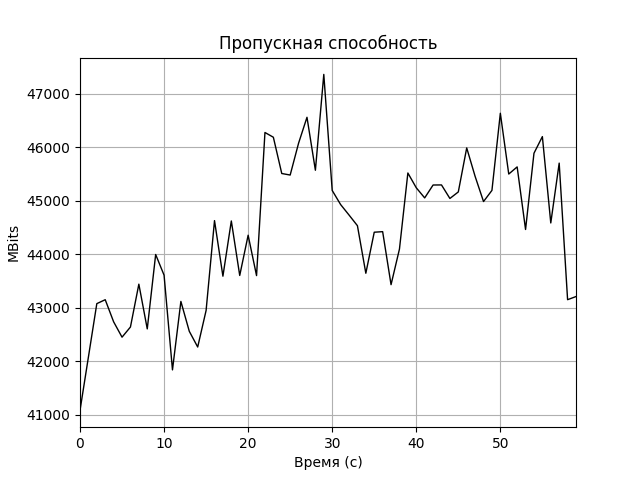
\includegraphics[width=0.7\textwidth,height=\textheight]{iperf_throughput.png}
\caption{График изменения значения пропускной способности с течением
времени}\label{fig:0019}
}
\end{figure}

\hypertarget{ux438ux441ux43fux43eux43bux44cux437ux43eux432ux430ux43dux438ux435-ux443ux442ux438ux43bux438ux442ux44b-iproute2-ux434ux43bux44f-ux43dux430ux441ux442ux440ux43eux439ux43aux438-ux438ux43dux442ux435ux440ux444ux435ux439ux441ux43eux432-ux441ux435ux442ux435ux432ux44bux445-ux44dux43bux435ux43cux435ux43dux442ux43eux432}{%
\chapter{Использование утилиты iproute2 для настройки интерфейсов
сетевых
элементов}\label{ux438ux441ux43fux43eux43bux44cux437ux43eux432ux430ux43dux438ux435-ux443ux442ux438ux43bux438ux442ux44b-iproute2-ux434ux43bux44f-ux43dux430ux441ux442ux440ux43eux439ux43aux438-ux438ux43dux442ux435ux440ux444ux435ux439ux441ux43eux432-ux441ux435ux442ux435ux432ux44bux445-ux44dux43bux435ux43cux435ux43dux442ux43eux432}}

\hypertarget{ux43eux431ux449ux438ux435-ux441ux432ux435ux434ux435ux43dux438ux44f}{%
\section{Общие
сведения}\label{ux43eux431ux449ux438ux435-ux441ux432ux435ux434ux435ux43dux438ux44f}}

\(\quad\)iproute2 --- это набор утилит для управления параметрами
сетевых устройств в ядре Linux. Утилиты разработаны в качестве
унифицированного интерфейса к ядру Linux, непосредственно управляющего
трафиком.

iproute2 заменил полный набор классических сетевых утилит UNIX, которые
ранее использовались для настройки сетевых интерфейсов, таблиц
маршрутизации и управления arp-таблицами: ifconfig, route, arp, netstat
и др., предназначенных для создания IP-туннелей. iproute2 предлагает
унифицированный синтаксис для управления аспектами сетевых интерфейсов.

Набор утилит включает в себя три основные программы:

\begin{itemize}
\tightlist
\item
  ip \autocite{ip} --- утилита для просмотра параметров и
  конфигурирования сетевых интерфейсов, сетевых адресов, таблиц и правил
  маршрутизации, ARP-таблиц, IP-туннелей, адресов multicast рассылки,
  маршрутизации multicast-пакетов;
\item
  tc \autocite{tc} --- утилита для просмотра и конфигурирования
  параметров управления трафиком, позволяющая управлять классификацией
  трафика, дисциплинами управления очередями для различных классов
  трафика либо целиком для сетевого интерфейса, что, в свою очередь,
  позволяет реализовать QoS в нужном для системы объёме:

  \begin{itemize}
  \tightlist
  \item
    разделение разных типов трафика по классам;
  \item
    назначение разных дисциплин обработки очередей трафика с разным
    приоритетом, механизмами прохождения очереди, ограничениями по
    скорости и т.п.;
  \end{itemize}
\item
  ss \autocite{ss} --- утилита для просмотра текущих соединений и
  открытых портов.
\end{itemize}

\hypertarget{ux443ux442ux438ux43bux438ux442ux430-tc}{%
\section{Утилита tc}\label{ux443ux442ux438ux43bux438ux442ux430-tc}}

\(\quad\)Утилита tc \autocite{tc} наиболее полезна для исследования, так
как она позволяет гибко настроить поведение контроля исходящего трафика.
Система контроля трафика состоит из следующих компонентов.

\begin{itemize}
\tightlist
\item
  Ограничения исходящего трафика (SHAPING). Когда трафик сформирован,
  его полоса пропускания начинает контролироваться. Ограничение может
  дать больше, чем уменьшение полосы пропускания - оно также
  используется для сглаживания пиков для более прогнозируемого поведения
  сети.
\item
  Планирования передачи пакетов (SCHEDULING). Это позволяет увеличить
  интерактивность исходящего трафика при гарантировании полосы
  пропускания для передачи данных большого объема. Такое упорядочение
  также называется приоритезацией и применяется для исходящего трафика.
\item
  Ограничения исходящего трафика (POLICING). Этот механизм позволяет
  ограничить количество пакетов или байт в потоке входящего трафика,
  соответствующих определенной классификации.
\item
  Отбрасывания (DROPPING). Трафик, превышающий установленную полосу
  пропускания, может быть отброшен как для входящего, так и исходящего
  трафика. Обработка трафика контролируется тремя типами объектов:
  очередями (qdiscs), классами и фильтрами. Обработка трафика
  контролируется тремя типами объектов: очередями (qdiscs), классами и
  фильтрами.
\end{itemize}

Для информации о tc используется команда \mintinline{bash}{tc help}.

\(\quad\)Дисциплина очереди --- это алгоритм обработки очереди сетевых
пакетов. Дисциплин на одном интерфейсе может быть задействовано
несколько, а непосредственно к интерфейсу крепится корневая дисциплина
(root qdisc). При этом каждый интерфейс имеет свою собственную корневую
дисциплину. Каждой дисциплине и каждому классу назначается уникальный
дескриптор (некоторый номер), который может использоваться последующими
инструкциями для ссылки на эти дисциплины и классы. Помимо исходящей
дисциплины, интерфейс так же может иметь и входящую дисциплину, которая
производит управление входящим трафиком. Дисциплины на интерфейсе
образуют иерархию, где в верху иерархии находится корневая дисциплина.
Сам интерфейс ничего не знает о дисциплинах, находящихся под корневой, а
поэтому работает только с ней.

Воспользуемся сетью Mininet из прошлой главы и с помощью tc выведем
информацию о дисциплине очереди на сетевом устройстве s1-eth0 (интерфейс
коммутатора, к которому подключен хост h1). Для этого воспользуемся
командой

\begin{minted}[breaklines]{bash}
tc -s qdisc show dev s1-eth1
\end{minted}

На рис. \ref{fig:0020} видно, что корневой дисциплиной очереди назначена
дисциплина noqueue. Данная дисциплина означает «отправляй мгновенно, не
ставь в очередь».

\begin{figure}
\hypertarget{fig:0020}{%
\centering
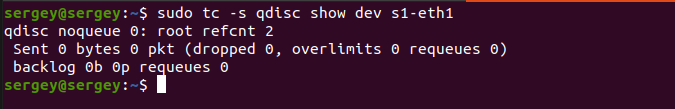
\includegraphics[width=0.7\textwidth,height=\textheight]{iproute_tc_qdisc_show_s1-eth1.png}
\caption{Информация о дисциплине очереди на сетевом устройстве
s1-eth0}\label{fig:0020}
}
\end{figure}

В выводе tc можно увидеть полезные для исследования данные:

\begin{itemize}
\tightlist
\item
  \emph{Sent 0 bytes 0 pkt (dropped 0, overlimits 0 requeues 0)} ---
  означает, что было отправлено 0 байт (0 пакетов), из которых 0 пакетов
  отброшено и 0 пакетов вышли за пределы лимита.
\item
  \emph{backlog 0b 0p requeues 0} --- размер очереди в байтах и пакетах.
\end{itemize}

Запомним параметр backlog: он будет полезен нам при сборе статистики.

\hypertarget{ux432ux438ux434ux44b-ux434ux438ux441ux446ux438ux43fux43bux438ux43d-ux43eux447ux435ux440ux435ux434ux435ux439}{%
\section{Виды дисциплин
очередей}\label{ux432ux438ux434ux44b-ux434ux438ux441ux446ux438ux43fux43bux438ux43d-ux43eux447ux435ux440ux435ux434ux435ux439}}

\hypertarget{ux431ux435ux441ux43aux43bux430ux441ux441ux43eux432ux44bux435-ux43eux447ux435ux440ux435ux434ux438}{%
\subsection{Бесклассовые
очереди}\label{ux431ux435ux441ux43aux43bux430ux441ux441ux43eux432ux44bux435-ux43eux447ux435ux440ux435ux434ux438}}

\(\quad\)Ниже перечислены виды бесклассовых очередей:

\begin{itemize}
\tightlist
\item
  pfifo/bfifo --- простейшие очереди без обработки, лишь реализующие
  принцип «First In, First Out» (первый вошел -- первый вышел).
  Ограничены в пакетах или байтах.
\item
  pfifo\_fast --- стандартная очередь ядра с `расширенным роутером'.
  Состоит из очереди с тремя потоками, учитывающей флаги типа услуги
  (Type of Service) и приоритет пакета.
\item
  RED --- Random Early Detection (случайное раннее обнаружение)
  симулирует физический затор, отбрасывая пакеты случайным образом при
  близком достижении заданной полосы пропускания. Хорошо подходит для
  приложений, требующих очень широкую полосу пропускания.
\item
  SFQ --- Stochastic Fairness Queueing (очередь равномерного случайного
  распределения пакетов) реорганизует трафик в очереди таким образом,
  что каждый `сеанс' (`session', виртуальная подочередь) получает право
  отправить пакет, а маркер переходит на следующий сеанс.
\item
  TBF --- Token Bucket Filter (фильтр буфера токенов) удерживает
  скорость передачи пакетов на примерно постоянном уровне (меньшем, чем
  реальная скорость интерфейса). Хорошо масштабируется для широких
  каналов.
\end{itemize}

Подробнее о видах бесклассовых очередей можно прочесть в \autocite{tc}.

\hypertarget{ux43eux447ux435ux440ux435ux434ux438-ux441-ux43aux43bux430ux441ux441ux430ux43cux438}{%
\subsection{Очереди с
классами}\label{ux43eux447ux435ux440ux435ux434ux438-ux441-ux43aux43bux430ux441ux441ux430ux43cux438}}

\(\quad\)Ниже перечислены виды очередей с классами \autocite{tc}:

\begin{itemize}
\tightlist
\item
  CBQ --- очередь, базирующаяся на классах (Class Based Queueing),
  реализует мощную иерархию классов. Поддерживает ограничения и
  приоритеты. Разделение осуществляется по времени простоя канала,
  вычисляемого на основании среднего размера пакета и полосы
  пропускания.
\item
  HTB --- очередь (Hierarchy Token Bucket --- иерархический буфер
  токенов) реализует мощную иерархию классов с упором на согласование с
  существующей практикой. HTB обеспечивает гарантированную полосу
  пропускания для классов, также позволяет устанавливать верхние пределы
  межклассового разделения очереди. Содержит объекты ограничения,
  базирующиеся на TBF, и может устанавливать приоритеты для классов.
\item
  PRIO --- очередь может разделять трафик между тремя полосами, которые
  являются очередями любого типа. При извлечении пакета из очереди
  вначале исследуется подочередь с большим приоритетом, если в последней
  нет пакетов для обработки, то выбирается очередь с более низким
  приоритетом. Для установки приоритета используются биты типа услуги
  (Type of Service).
\end{itemize}

\hypertarget{ux43fux440ux438ux43cux435ux440-ux43fux43eux441ux442ux440ux43eux435ux43dux438ux44f-ux438ux435ux440ux430ux440ux445ux438ux438-ux434ux438ux441ux446ux438ux43fux43bux438ux43d}{%
\section{Пример построения иерархии
дисциплин}\label{ux43fux440ux438ux43cux435ux440-ux43fux43eux441ux442ux440ux43eux435ux43dux438ux44f-ux438ux435ux440ux430ux440ux445ux438ux438-ux434ux438ux441ux446ux438ux43fux43bux438ux43d}}

\(\quad\)Построим простую топологию сети. Пусть, у нас имеется 2 хоста
соединенные с сетью. Сеть состоит из двух коммутаторов с разными
скоростями передачи данных. Назовем сетевые элементы как h1
(хост-передатчик), h2 (хост-приемник), s1 (коммутатор, соединенный с h1)
и s2(коммутатор, соединенный с h2). Тогда сеть будет иметь следующие
характеристики:

\begin{itemize}
\tightlist
\item
  скорость передачи данных от s1 к h1 равна 100 Мбит/c;
\item
  скорость передачи данных от s1 к s2 равна 100 Мбит/c;
\item
  скорость передачи данных от s2 к h2 равна 50 Мбит/c;
\item
  задержка распространения между h1 и s1 равна 30 мс +- 7 мс;
\item
  задержка распространения между s1 и s2 равна 30 мс +- 7 мс;
\item
  процент потерь пакетов на каждом сетевом соединении равен 0.01\%;
\item
  дисциплиной очереди, которая установлена на интерфейсе s2-eth2, будет
  pfifo с максимальным количеством пакетов 30.
\end{itemize}

Скорость передачи на интерфейсе можно ограничить с помощью дисциплины
tbf, а эмулировать задержки распространения и потери мы будем с помощью
дисциплины NetEm. NetEm обеспечивает функциональность сетевой эмуляции
для тестирования протоколов, имитируя свойства глобальных сетей.

\begin{enumerate}
\def\labelenumi{\arabic{enumi}.}
\tightlist
\item
  Откроем MiniEdit и создадим простую топологию сети (рис.
  \ref{fig:0030}).
\end{enumerate}

\begin{figure}
\hypertarget{fig:0030}{%
\centering
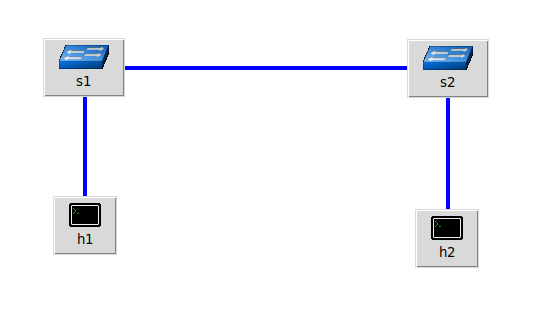
\includegraphics[width=0.7\textwidth,height=\textheight]{iproute_net_topo.png}
\caption{Топология сети}\label{fig:0030}
}
\end{figure}

\begin{enumerate}
\def\labelenumi{\arabic{enumi}.}
\setcounter{enumi}{1}
\tightlist
\item
  Запустим сеть.
\item
  Введем следующие команды tc:
\end{enumerate}

\begin{minted}[breaklines,linenos]{bash}
  sudo tc qdisc replace dev s1-eth2 root handle 10: tbf rate 100mbit burst 50000 limit 150000
  sudo tc qdisc add dev s1-eth2 parent 10: handle 20: netem loss 0.01% delay 30ms 7ms distribution normal
  sudo tc qdisc replace dev s1-eth1 root handle 10: tbf rate 100mbit burst 50000 limit 150000
  sudo tc qdisc add dev s1-eth1 parent 10: handle 20: netem loss 0.01% delay 30ms 7ms distribution normal
  sudo tc qdisc replace dev s2-eth2 root handle 10: tbf rate 50mbit burst 25000 limit 75000
  sudo tc qdisc add dev s2-eth2 parent 10: handle 15: pfifo limit 30
  sudo tc qdisc replace dev s2-eth1 root handle 10: tbf rate 50mbit burst 25000 limit 75000
  \end{minted}

Любая команда добавления дисциплины на интерфейс, работающая с
бесклассовыми дисциплинами, имеет вид:

\begin{minted}[breaklines]{bash}
  tc qdisc [add/replace] dev [interface] [root/parent num] handle [number]: [Queue Discipline] [discipline parameters]
  \end{minted}

Параметры команды:

\begin{itemize}
\tightlist
\item
  {[}add/replace{]} --- выбирается в зависимости от иерархии дисциплин.
  Если дисциплина еще не назначена --- ставим add, если требуется
  заменить существующую дисциплину --- ставим replace;
\item
  {[}interface{]} --- фактический сетевой интерфейс устройства;
\item
  {[}root/parent num{]} --- выбирается в зависимости от иерархии
  дисциплин. Если дисциплина должна быть назначена как корневая ---
  ставим root, если дисциплина должна прикрепиться к родителю --- ставим
  parent с дескриптором родителя;
\item
  {[}number{]} --- дескриптор, который мы назначаем на дисциплину;
\item
  {[}Queue Discipline{]} --- название дисциплины;
\item
  {[}discipline parameters{]} --- параметры дисциплины.
\end{itemize}

TBF --- дисциплина, построенная на понятии токена и заполненности
некоторого буфера, называемого ведром». Данные поступают на вход
алгоритма, токены генерируются и поступают в «ведро». Если токен имеется
в «ведре», то данные проходя на интерфейс и отправляются в сеть. Если
«ведро» пусто, то пакеты ставятся в очередь. По достижению некоторого
лимита очереди пакеты отбрасываются.

Параметры tbf:

\begin{itemize}
\tightlist
\item
  rate --- фактическая скорость, с которой генерируются токены;
\item
  burst --- количество байтов, которое может поместиться в ведре;
\item
  limit --- размер очереди.
\end{itemize}

Параметры netem:

\begin{itemize}
\tightlist
\item
  loss --- процент потерь на соединении;
\item
  delay --- задержка распространения. В нашем примере запись \emph{delay
  30ms 7ms distribution normal} означает, что задержка равна 30 мс, при
  этом это значение варьируется от 23 до 37 мс с вероятностью, заданной
  нормальным распределением.
\end{itemize}

\begin{enumerate}
\def\labelenumi{\arabic{enumi}.}
\setcounter{enumi}{3}
\tightlist
\item
  Запустим iPerf-клиет и iPerf-сервер (рис. \ref{fig:0031}). Запишем
  данные в файл json и построим графики сетевых характеристик.
\end{enumerate}

\begin{figure}
\hypertarget{fig:0031}{%
\centering
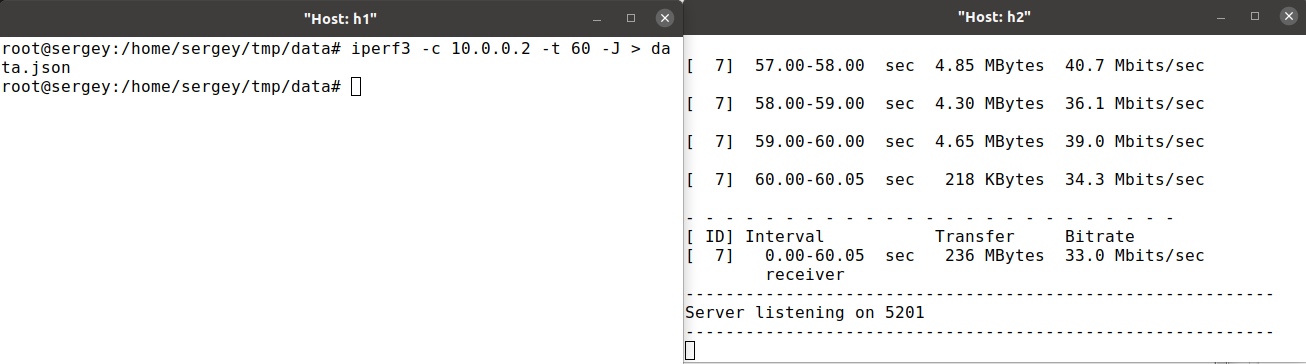
\includegraphics[width=0.8\textwidth,height=\textheight]{iproute_monitor.png}
\caption{Мониторинг сети}\label{fig:0031}
}
\end{figure}

\begin{enumerate}
\def\labelenumi{\arabic{enumi}.}
\setcounter{enumi}{4}
\tightlist
\item
  Рассмотрим, как изменилось поведение нашей сети в сравнении с из
  прошлым разделом, где рассматривалась идеальная сеть без заданных
  сетевых параметров (потерь, задержек, максимальной скорости передачи).
\end{enumerate}

Окно перегрузки (рис. \ref{fig:0032}) достаточно долго не может найти
оптимальное значение, так как происходят частые потери из-за увеличения
размера очереди на коммутаторе. Так как по умолчанию на рабочей машине
стоит алгоритм для работы с перегрузками TCP Reno, то видно что график
принимает пилообразные очертания.

\begin{figure}
\hypertarget{fig:0032}{%
\centering
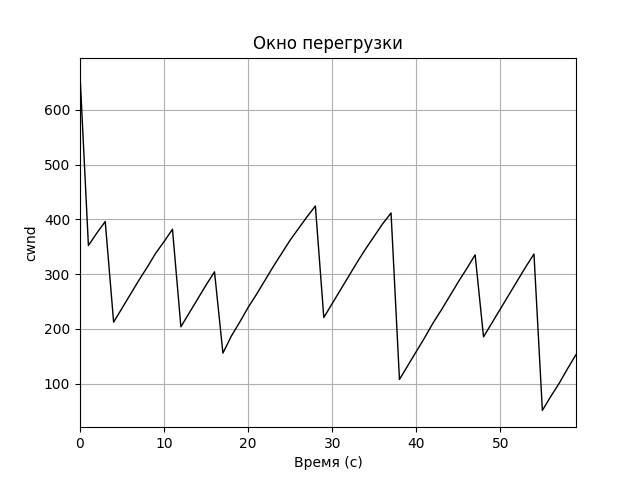
\includegraphics[width=0.7\textwidth,height=\textheight]{iproute_cwnd.png}
\caption{График изменения значения окна перегрузки TCP
Reno}\label{fig:0032}
}
\end{figure}

На рис. \ref{fig:0033} приведен график изменения значения количества
повторно переданных данных с течением времени --- появились потери
пакетов на соединении, причем, достаточно частые.

\begin{figure}
\hypertarget{fig:0033}{%
\centering
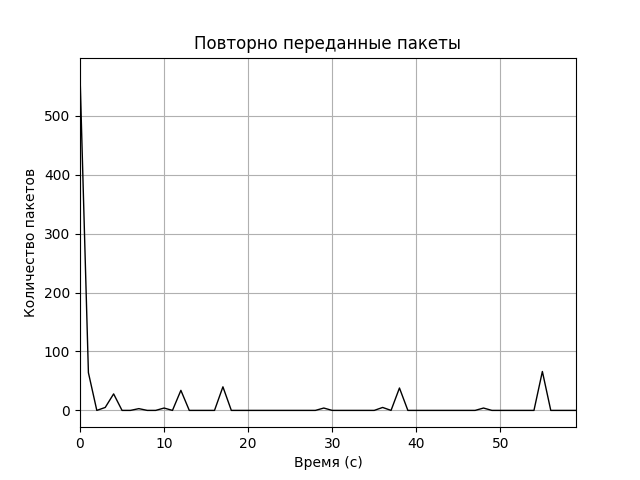
\includegraphics[width=0.7\textwidth,height=\textheight]{iproute_retransmits.png}
\caption{График изменения количества повторно переданных
данных}\label{fig:0033}
}
\end{figure}

Среднее значение RTT (рис. \ref{fig:0034}) сильно увеличилось (0.04 мс
против 60 мc), что связано с мгновенной отправкой данных без задержки в
очереди.

\begin{figure}
\hypertarget{fig:0034}{%
\centering
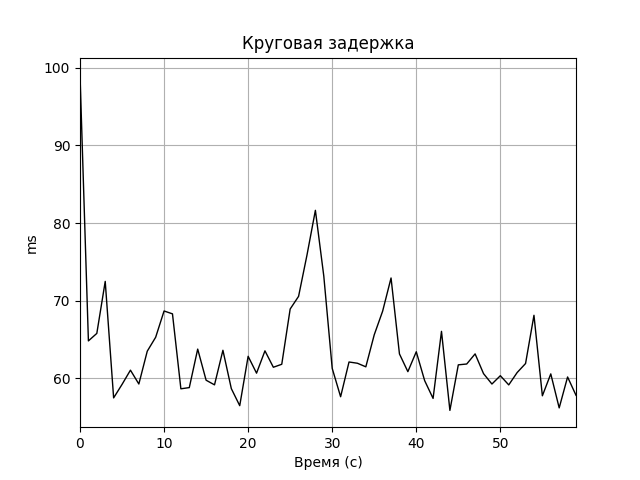
\includegraphics[width=0.68\textwidth,height=\textheight]{iproute_rtt.png}
\caption{График изменения значения RTT с течением
времени}\label{fig:0034}
}
\end{figure}

Пропускная способность (рис. \ref{fig:0035}) колеблется от 0 Мбит/с до
70 мбит/c из-за искусственного ограничения скорости передачи, потерь в
сети и задержек распространения.

\begin{figure}
\hypertarget{fig:0035}{%
\centering
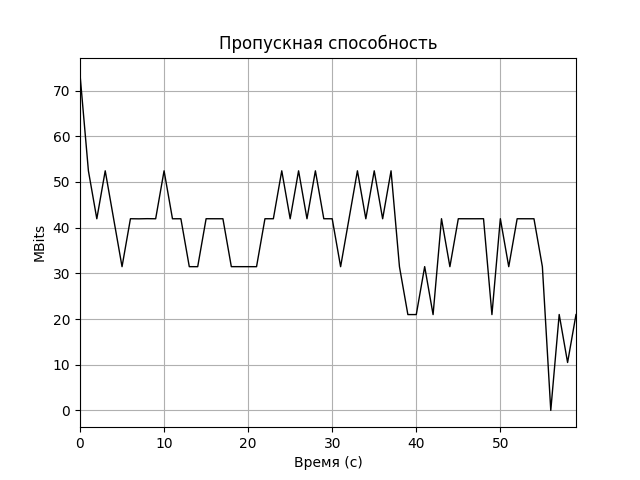
\includegraphics[width=0.7\textwidth,height=\textheight]{iproute_throughput.png}
\caption{График изменения значения пропускной
способности}\label{fig:0035}
}
\end{figure}

\hypertarget{ux438ux437ux43cux435ux440ux435ux43dux438ux435-ux440ux430ux437ux43cux435ux440ux430-ux43eux447ux435ux440ux435ux434ux438-ux43dux430-ux434ux438ux441ux446ux438ux43fux43bux438ux43dux435}{%
\section{Измерение размера очереди на
дисциплине}\label{ux438ux437ux43cux435ux440ux435ux43dux438ux435-ux440ux430ux437ux43cux435ux440ux430-ux43eux447ux435ux440ux435ux434ux438-ux43dux430-ux434ux438ux441ux446ux438ux43fux43bux438ux43dux435}}

\(\quad\)Некоторые сетевые характеристики мы уже успели рассмотреть в
прошлой главе. Однако, иногда для анализа работы сети оказывается
полезной еще одна характеристика, которую мы не можем измерить с помощью
iPerf, так как данных по ней попросту нет ни на хосте, ни на сервере.
Речь идет о длине очереди на сетевом устройстве.

Задача разработчиков сети --- достигнуть оптимальной скорости передачи
данных с минимально возможной задержкой. Одним из факторов, который
сказывается на это, является очередь на коммутаторах/маршрутизаторах.
Буфер в коммутаторе (место, куда поступают пакеты и становятся в очередь
на обслуживание) помогает не потерять пакеты, если имеет место высокая
интенсивность поступления трафика. Если сеть работает на пределе,
очередь коммутатора/маршрутизатора будет заполнена и пакеты начнут
теряться. Чем длиннее очередь, тем больше задержка, что в свою очередь
сильно сказывается на общей пропускной способности сети.

Реакцию очереди на изменение конфигураций передачи данных можно измерить
и в зависимости от результатов подстроить другие параметры для
достижения лучшей работы сети в целом. Например, изменив алгоритм работы
с перегрузками на хостах, или дисциплину очереди, можно достичь лучшей
производительности сети.

Для измерения длины очереди полезным окажется вывод статистики tc.
Запись backlog указывает на размер очереди дисциплины в байтах и
пакетах. Это статистику можно снять и измерять каждый промежуток времени
с помощью функции на любом языке программирования. Функция записывает
время и размер очереди в файл, с помощью которого легко построить
график, например, в gnuplot.

Напишем функцию, которая замеряет размер очереди с заданным интервалом
времени. Диграмма активностостей для такой функции приведена на рис.
\ref{fig:0036}. С помощью скрипта на языке программирования python
(\protect\hyperlink{appendix2}{см. приложение В}) построим график
изменения длины очереди на интерфейсе \ref{fig:0037}.

Настройки сети аналогичны сети из прошлой главы (включая настройки
qdisc).

\begin{figure}
\hypertarget{fig:0036}{%
\centering
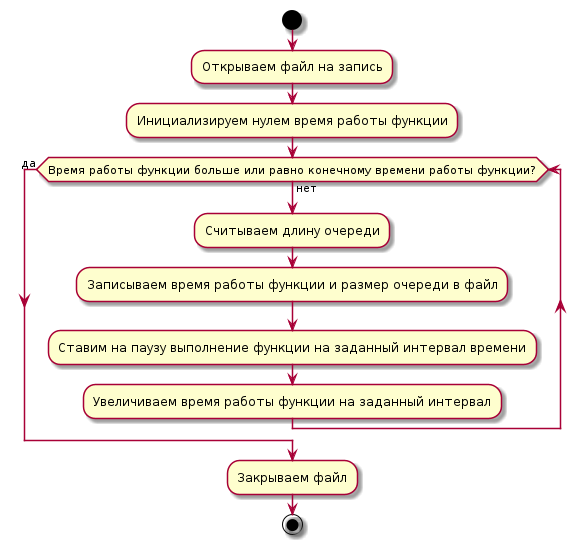
\includegraphics[width=0.9\textwidth,height=\textheight]{iproute_act_dia.png}
\caption{Диаграмма активностей для функции замеров длины
очереди}\label{fig:0036}
}
\end{figure}

\begin{figure}
\hypertarget{fig:0037}{%
\centering
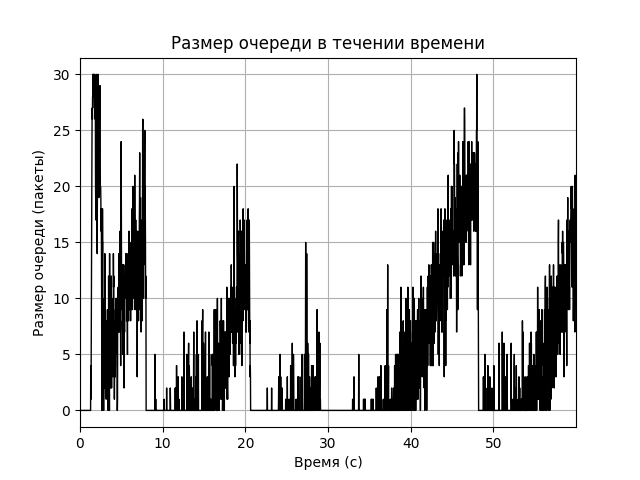
\includegraphics[width=0.7\textwidth,height=\textheight]{iproute_queue_len.png}
\caption{График изменения длины очереди на интерфейсе
s2-eth2}\label{fig:0037}
}
\end{figure}

На графике видно, что в определенные моменты времени длина очереди или
возрастает, или убывает. Связано это с алгоритмом TCP Reno. При высокой
загруженности канала связи увеличивается длина очереди и, как следствие,
RTT. В момент, когда RTT переходит за допустимую норму, источник
уменьшает окно перегрузки, что влечет за собой уменьшение битрейта и
длины очереди.

\hypertarget{ux437ux430ux43aux43bux44eux447ux435ux43dux438ux435}{%
\chapter*{Заключение}\label{ux437ux430ux43aux43bux44eux447ux435ux43dux438ux435}}
\addcontentsline{toc}{chapter}{Заключение}

\(\quad\)В ходе курсовой работы мы научились моделировать простые
виртуальные сети с помощью программы Mininet, рассмотрели технологии,
которые помогают в сборе данных сетевых характеристик, оценили
производительность сетей и рассмотрели способы визуализации полученных
данных. Mininet предоставляет разработчикам быстрый и дешевый в
построении испытательный полигон, в котором можно проектировать и
отлаживать сетевые программы, что является большим плюсом для
бизнес-сегмента.

Мониторинг сетевых характеристик передачи данных является неотъемлемой
частью при проектировании сетей и сетевых программ. Умея анализировать
данные сетевых характеристик, можно строить гибкие решения, которые
позволяют получить максимальную производительность сетевого ресурса.

\appendix

\printbibliography[heading=bibintoc]

\appendix

\hypertarget{appendix1}{%
\chapter{Построение графиков сетевых характеристик из полученных данных
iPerf3}\label{appendix1}}

\(\quad\)Имея данные в формате json их обработка на языке
программирования python сводится к тривиальной. Первым делом мы
подключаем модуль json к программе, с помощью метода load загружаем
данные переменную. На выходе у нас имеется готовый список данных,
обработка которых представляет собой выбор по ключевому полю данных и их
запись в нужную переменную. Код для функции обработки данных представлен
ниже.

\begin{minted}
[
frame=lines,
framesep=2mm,
baselinestretch=1.2,
fontsize=\footnotesize,
linenos
]
{python}
'''
    Функция обработки данных iPerf.
    Данные обрабатываются из предположения, что нас
    интересуют только данные, перечисленные в 
    словаре y. Функция возвращает словарь [x,y].
'''
def parse_netstat_file(net_data_file):
    raw_data = json.load(net_data_file)
    x = []
    y = {
        "bytes": [[], 
        {"title": "Количество переданных байт", "x": "Время (с)", "y": "MB"}],
        "cwnd": [[], 
        {"title": "Окно перегрузки", "x": "Время (с)", "y": "cwnd"}],
        "MTU": [[], 
        {"title": "Максимальный размер пакета", "x": "Время (с)", "y": "B"}],
        "retransmits": [[], 
        {"title": "Повторно переданные пакеты", "x": "Время (с)", "y": "Количество пакетов"}],
        "rtt": [[], 
        {"title": "Круговая задержка", "x": "Время (с)", "y": "ms"}],
        "rttvar": [[], 
        {"title": "Отклонение круговой задержки", "x": "Время (с)", "y": "ms"}],
        "throughput": [[], 
        {"title": "Пропускная способность", "x": "Время (с)", "y": "MBits"}]
    }
    '''
        Цикл считывания данных из json-файла.
        В список x сохраняются временные данные, а 
        в словарь y - все остальные. Характеристи для y
        нормируются в зависимости от требуемой 
        шкалы измерения данных.
    '''
    for i in raw_data["intervals"]:
        tmp_data = i["streams"][0]
        x.append(tmp_data["start"])
        y["bytes"][0].append(tmp_data["bytes"] / 1024 / 1024)
        y["cwnd"][0].append(tmp_data["snd_cwnd"] / 1024)
        y["MTU"][0].append(tmp_data["pmtu"])
        y["retransmits"][0].append(tmp_data["retransmits"])
        y["rtt"][0].append(tmp_data["rtt"] / 1000)
        y["rttvar"][0].append(tmp_data["rttvar"] / 1000)
        y["throughput"][0].append(tmp_data["bits_per_second"] / 1000000)
    return [x, y]
\end{minted}

Получив обработанные данные, мы можем построить графики. Код для функции
построения графиков представлен ниже.

\begin{minted}
[
frame=lines,
framesep=2mm,
baselinestretch=1.2,
fontsize=\footnotesize,
linenos
]
{python}
'''
    Функция построения графиков сетевых характеристик.
    На вход поступает список значений, где первый элемент -
    время, а второй элемент - список значений сетевых 
    характеристик.
    Графики сохраняются в заданном формате 
    (параметр plot_format) и в заданную 
    директорию (параметр folder)
'''
def plot_net_stats(stats, plot_format, folder):
    x_stats, y_stats = stats
    for i in y_stats:
        plt.plot(x_stats, y_stats[i][0], 'k', linewidth=1)
        plt.grid()
        plt.xlim(xmin=0, xmax=x_stats[-1])
        plt.xlabel(y_stats[i][1]["x"])
        plt.ylabel(y_stats[i][1]["y"])
        plt.title(y_stats[i][1]["title"])
        plt.savefig("{}{}.{}".format(folder, i, plot_format))
        plt.clf()
\end{minted}

Теперь мы можем соединить эти функци воедино в скриптовом файле, выбрать
целевой файл, передать параметры для функций и построить графики сетевых
характеристик.

\hypertarget{appendix2}{%
\chapter{Построение графика изменения длины очереди на сетевом
интерфейсе}\label{appendix2}}

\(\quad\)Файл данных для очереди представляет собой плоский файл, в
котором имеется две колонки: время в секундах и размер очереди в
пакетах, разделенные пробелом. Все, что нам нужно сделать - это отделить
данные друг от друга, запись их в нужные структуры данных и позже
данными для построения графика. Пример кода для функции обработки данных
размера очереди представлен ниже.

\begin{minted}
[
frame=lines,
framesep=2mm,
baselinestretch=1.2,
fontsize=\footnotesize,
linenos
]
{python}
'''
    Функция обработки данных изменения
    длины очереди. Разделяем данные из 
    предположения, что 1-й элемент - 
    значение времи (значение заносится в список x), 
    2-й элемент - длина очереди (значение 
    заносится в список y). 
    Функция возвращает список [x,y]
'''
def parse_queue_len(qlen_data_file):
    x_stats = []
    y_stats = []
    for line in qlen_data_file:
        line = line.split(" ")
        x_stats.append(float(line[0]))
        y_stats.append(float(line[1]))
    return [x_stats, y_stats]

\end{minted}

Имея список значений x и список значений y, построим график изменения
длины очереди.

\begin{minted}
[
frame=lines,
framesep=2mm,
baselinestretch=1.2,
fontsize=\footnotesize,
linenos
]
{python}
'''
    Функция построения графика изменения длины очереди.
    На вход поступает список значений, где первый элемент -
    время, а второй элемент - список значений длины очереди.
    Графики сохраняются в заданном формате 
    (параметр plot_format) и в заданную 
    директорию (параметр folder)
'''
def plot_queue_len(stats, plot_format, folder):
    x_stats, y_stats = stats
    plt.plot(x_stats, y_stats, 'k', linewidth=1)
    plt.grid()
    plt.xticks(np.arange(0.0, x_stats[-1], step=10.0))
    plt.xlim(xmin=0, xmax=x_stats[-1])
    plt.xlabel("Время (с)")
    plt.ylabel("Размер очереди (пакеты)")
    plt.title("Размер очереди в течении времени")
    plt.savefig("{}queue_len.{}".format(folder, plot_format))
\end{minted}

Теперь мы можем соединить эти функци воедино в скриптовом файле, выбрать
целевой файл, передать параметры для функций и построить график
изменения длины очереди на сетевом интерфейсе.

\end{document}
